You are considering implementing the proportional control system shown below. The desired specifications are a settling time of $\ts \leq 2$ s and a rise time of  $\tr \leq 0.5$ s. 
\begin{center}
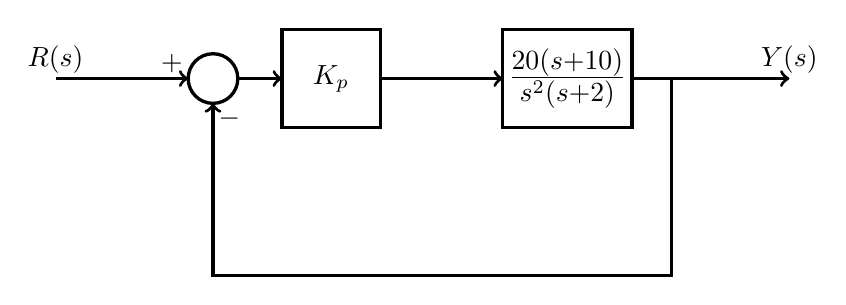
\begin{tikzpicture}[scale=1,inner sep=0pt,outer sep=0pt,very thick,
sysblock/.style={draw,rectangle,inner sep=2pt,minimum width=1.25cm,minimum height=1.25cm,very thick}]
\draw (2,0) node[draw,circle] (sum1) {$\rule{0pt}{18pt}$};
\draw (3.5,0) node[sysblock] (Kp) { $K_{p}$};
\draw (6.5,0) node[sysblock] (G) {\Large $\frac{20(s+10)}{s^2\left(s+2\right)}$};
\draw[->] (0,0) node[above=2pt] {$R(s)$} -- (sum1.180) node[above left=2pt] {$+$};
\draw[->] (sum1.0) --  (Kp);
\draw[->] (Kp) -- (G.180);
\draw[->] (G.0) -- ++(2,0) node[above=2pt] {$Y(s)$};
\draw[->] (G.0) ++(0.5,0) -- ++(0,-2.5) -| (sum1.-90) node[below right=2pt] {$-$};
\end{tikzpicture}
\end{center}

\begin{enumerate}[(a)]
\setlength{\itemsep}{0.5in}
\setlength{\parskip}{0pt}
\setlength{\parsep}{0pt}
\item Sketch the appropriate region in the complex plane where the dominant closed loop  poles should lie for all specifications to be met
\begin{center}
\begin{tikzpicture}[scale=1.0]
\draw[->] (0,0) -- (8,0) node[above]{Re$\{s\}$};
\draw[->] (6,-3) -- (6,3) node[right]{Im$\{s\}$};
\draw[-]  (.1,.1) -- ++(0,-.2) node[below] {$-10$};
\draw[-]  (6.1,2.6) node[right] {$j5$} -- ++(-.2,0) ;
\draw[-]  (6.1,-2.6) node[right] {$j5$} -- ++(-.2,0) ;

\end{tikzpicture}
\end{center}
\item By sketching the root locus (also on the above axis) determine whether all closed loop poles can be placed in the region sketched in part (a) for some value of $K_{p}$. 
\end{enumerate}

